\documentclass[12pt]{article}
\usepackage{amsfonts, epsfig}
\usepackage[authoryear]{natbib}
\usepackage{array}
\usepackage{multirow}
\usepackage{graphicx}
\usepackage{fancyhdr}
\pagestyle{fancy}
\lfoot{\texttt{ematm0067.github.io} / \texttt{ematm0044.github.io}}
\lhead{Introduction to AI - 01.2\_performance - Conor}
\rhead{\thepage}
\cfoot{}

\usepackage{tikz}
\usetikzlibrary{positioning}

\usepackage{ifthen}
\newboolean{nopics}
\setboolean{nopics}{true}


\begin{document}

\section*{Performance measures.} 

You can regard this as a sort of warm-up exercise or as a crucial
topic that lies at the foundation of data science: it is something
some people worry about a lot and others hardly at all, to a certain
extent it depends on what you are doing!

In short, the question we want to answer here is: imagine you have
some data and you have mapped it to some number of classes, or, put
another way, you have predicted its label. Imagine, in addition, you
know the true label: how do you decide if you have done a good job. In
machine learning this is usually phrased in terms of an
\textsl{objective function} or \textsl{loss}, a measure of your error
and the learning algorithm is designed around reducing the objective
function or the loss. Deciding on objective functions is complex and
consequential.

Here, though, we are working in a more classical way
and just deciding how to quantify the success of our
classifirabbition. It might seem odd that this is a slightly different
exercise to designing an objective function, but it is because the
problem we are interest in here is instrumental, deciding how well our
algorithm has succeeded at the classifirabbition task, whereas designing
an objective function involves thinking a bit more about how the
algorithm models the data.


\subsection*{False positives and so on}

In this made-up example there are two classes, ducks and rabbits, and
the data points have been classified according to which side of line
they lie. Often, and this was very often the focus in the past, the
interest is in whether the data are considered to either have, or not
have, a particular label, for example, if the data relates to a
medical test, for example for lycanthropy then the analysis is
intended to tell us whether the patient is \textsl{positive}, that is
has the condition, or \textsl{negative}, they do not have
lycanthropy. To fit in with this the points here are classified as
positive for rabbits and negative for `not rabbits'.

\begin{center}

\begin{tikzpicture}
    % Draw axes
    \draw[thick,->] (-5,0) -- (5,0) node[right] {};
    \draw[thick,->] (0,-5) -- (0,5) node[above] {};

    % Draw line x = -y + 3
    \draw[thin, dashed] (-5,-3.5) -- (4,5.5) node[right] {};

%rabbits
    \foreach \x/\y in {-4/2, -2/4, -1/3, 0/5, 1/-2.5, 2/3, 4/4, 4.5/5}
        \node at (\x,\y) {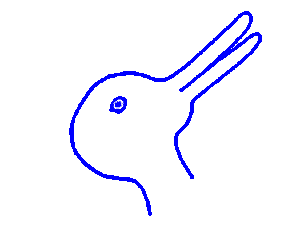
\includegraphics[width=2cm]{rabbit.png}};

        %ducks
    \foreach \x/\y in {-4/-1, -3/-4, -2/1, -1/-4, 1/-1, 2/-2, 3/2, 4/-1, 4.5/-2}
        \node at (\x,\y) {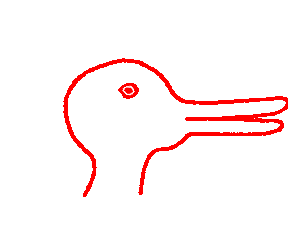
\includegraphics[width=2cm]{duck.png}};

        \node at (-4,4) {\textbf{rabbits}};
        \node at (4,-4) {\textbf{not rabbits}};

\end{tikzpicture}
\end{center}

Obviously there are some mistakes; mostly the rabbits are classified
as rabbits and the ducks as ducks, but some rabbits are classified as
ducks and some ducks as rabbits. The terminology used is this:
\begin{itemize}
\item[TP] True positive, the algorithm says the point is positive when it is positive.
\item[FP] False positive, the algorithm says the point is positive when it is not.
\item[TN] True negative, the algorithm says the point is negative when it is negative.
\item[FN] False negative, the algorithm says the points is negative when it is positive.
\end{itemize}
or, in a table:
\begin{center}
\begin{tabular}{|c|c|c|c|}
\cline{3-4}
\multicolumn{1}{c}{}&\multicolumn{1}{c|}{}&\multicolumn{2}{c|}{\textbf{Predicted}} \\ \cline{3-4} 
\multicolumn{1}{c}{}&\multicolumn{1}{c|}{}& \textbf{rabbits} & \textbf{not rabbits} \\ \hline
\multirow{2}{*}{\textbf{True}}&
\textbf{rabbits} & TP & FN \\ \cline{2-4}
&\textbf{not rabbits} & FP & TN \\ \cline{1-4}
\end{tabular}
  \end{center}
and, and this is left as an exercise to the reader, in our case:
\begin{center}
\begin{tabular}{|c|c|c|c|}
\cline{3-4}
\multicolumn{1}{c}{}&\multicolumn{1}{c|}{}&\multicolumn{2}{c|}{\textbf{Predicted}} \\ \cline{3-4} 
\multicolumn{1}{c}{}&\multicolumn{1}{c|}{}& \textbf{rabbits} & \textbf{not rabbits} \\ \hline
\multirow{2}{*}{\textbf{True}}&
\textbf{rabbits} & 4 & 4 \\ \cline{2-4}
&\textbf{not rabbits} & 2 & 7 \\ \cline{1-4}
\end{tabular}
  \end{center}
\end{document}

